I chatbot, assistenti virtuali, sono tra gli strumenti che, grazie ai progressi nel campo dell'intelligenza artificiale, stanno riscuotendo notevole successo per aiutare e guidare l'utente nell'utilizzo di nuove tecnologie.

La Bookmark s.r.l. è una società informatica che sviluppa software gestionali web e, come tutte le aziende del settore, deve, per contratto, garantire la necessaria assistenza ai propri clienti. 
%
Tuttavia, una considerevole quantità di richieste di assistenza potrebbe essere smaltita "a monte" mediante l'uso di un assistente virtuale che, riuscendo ad interpretare la domanda dell'utente, è in grado di guidarlo e fornire una prima rapida forma di assistenza.

Scopo di questo tirocinio era quindi quello di integrare un chatbot all'interno di una piattaforma gestionale finalizzato ad aziende di distribuzione e retail già esistente e funzionante.

Il chatbot è stato integrato all'interno di Active Demand, una piattaforma gestionale web che integra i principali processi commerciali: contratti, politiche di \textit{pricing}, gestione magazzino e promozioni.

Il chatbot utilizzato è di tipo ad "oracolo".
%
La differenza sostanziale con un chatbot procedurale è che l'utente è guidato, sin dall'inizio, a compiere un insieme di scelte, viene cioè incanalato lungo uno degli $n$ percorsi prefissati in fase di sviluppo, mentre un chatbot di tipo ad "oracolo" è addestrato a riconoscere ed interpretare il senso della frase scritta dall'utente e a rispondere in modo adeguato.
%
Questo ultimo approccio consentirebbe quindi, teoricamente, se configurato opportunamente, di poter rispondere a qualsiasi tipo di domanda o input dell'utente.

\begin{figure}%
    \centering
    \subfloat[\centering Esempio di chatbot procedurale - TOBi (Vodafone) ]{{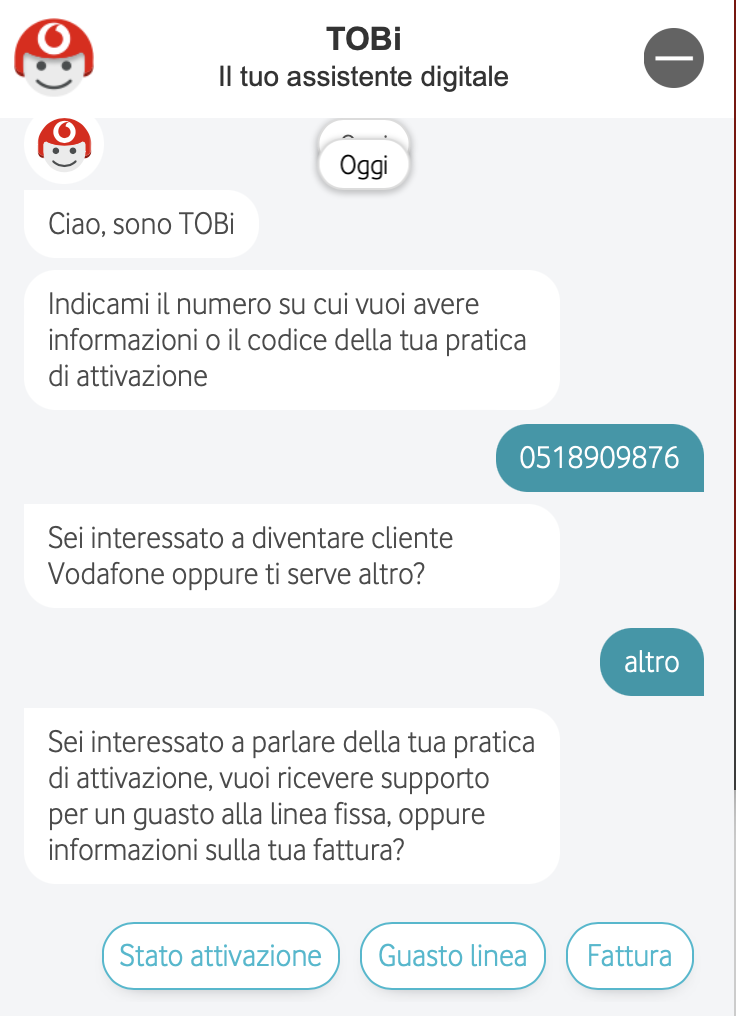
\includegraphics[width=5cm]{./img/chatbot-procedurale.png} }}%
    \qquad
    \subfloat[\centering Esempio di chatbot ad oracolo]{{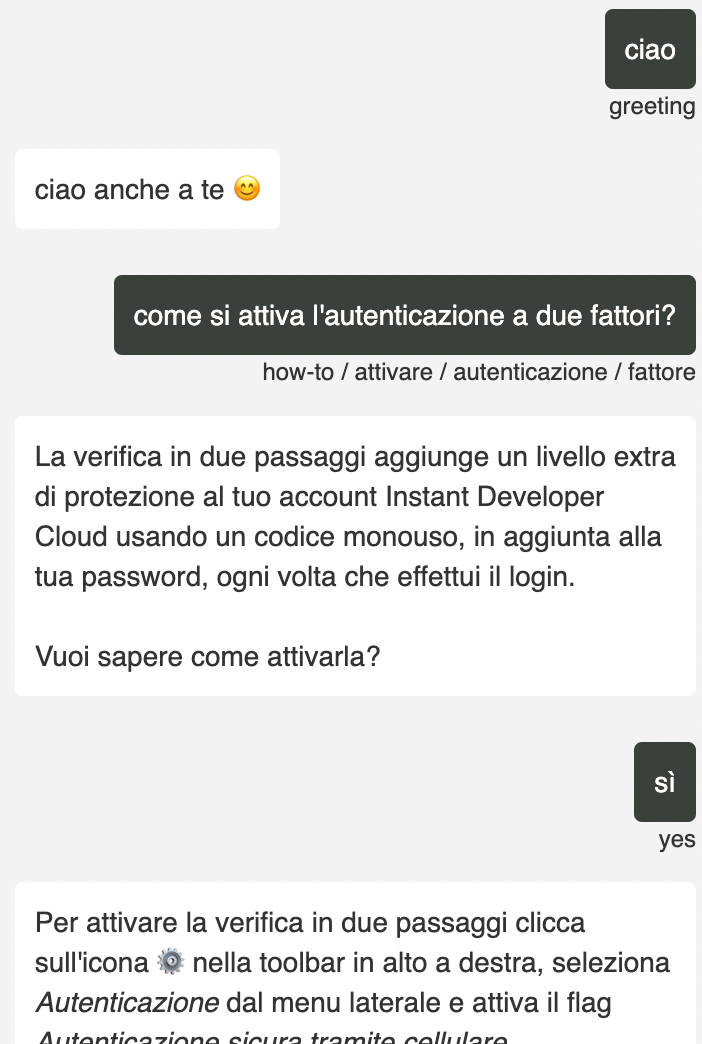
\includegraphics[width=5cm]{./img/chatbot-oracolo.png} }}%
    \caption{Esempi di chatbot}%
    \label{fig:example}%
\end{figure}
